\documentclass[main.tex]{subfiles}
\begin{document}


\section{Детерминистическая квантовая механика}\label{ch4}

\subsection{Вступление}\label{ch4.1}

Большинство попыток сформулировать теории скрытых переменных в существующей в настоящее время литературе состоят из некоторой модификации реальной квантовой теории и замены обычной классической физики каким-то стохастическим формализмом. За этим всегда стоит идея, что квантовая механика настолько отличается от классической физики, что некоторые глубокие модификации стандартных процедур кажутся необходимыми.

В подходе, отстаиваемом здесь, утверждается, что то, что мы называем детерминированной квантовой механикой, намного ближе к стандартным процедурам, чем обычно считается возможным.

\textit{Детерминированная квантовая механика не является ни модификацией стандартной квантовой механики, ни модификацией классической теории. Она находится на стыке этих двух теорий.}

Это поперечное сечение намного больше и перспективнее, чем обычно думают. Мы можем сформулировать теорию двумя способами: начиная с традиционной квантовой механики или начиная с совершенно классической. Мы уже видели в предыдущих частях этой работы, что это значит; здесь мы резюмируем.

Исходя из традиционной квантовой механики, детерминированная квантовая механика представляет собой небольшое подмножество всех квантовых теорий: \textit{мы постулируем существование очень особого базиса в гильбертовом пространстве: онтологического базиса}. Онтологический базис - это базис, с помощью которого уравнение Шредингера отправляет базисные элементы в другие базисные элементы в достаточно плотные моменты времени.

Весьма вероятно, что для онтологического базиса будет много разных вариантов (часто связанных преобразованиями симметрии), и будет трудно решить, какой из них является <<реальным>>. Любой из этих вариантов выбора для нашего онтологического базиса будет служить нашей цели, но только один из них будет <<истинным>>, и нам будет практически невозможно решить, какой именно.

Не будем сильно переживать по этому поводу. Поиск квантовых теорий, которые имеют онтологический базис, будет важным и трудным занятием. Мы надеемся, что это упражнение может привести к новым теориям, которые могут помочь развитию физики элементарных частиц и квантовой гравитации. Также это может помочь нам найти специальные теории космологии.

Наше определение онтологического базиса намеренно немного расплывчато. Мы не указываем, насколько плотными должны быть моменты времени, и точно не указываем, как определяется время; в специальной теории относительности мы можем выбирать различные системы отсчета, где время означает что-то другое. В общей теории относительности необходимо указать поверхности Коши, которые определяют временные срезы. Действительно важно то, что онтологический базис позволяет определить значимое подмножество наблюдаемых как операторы, диагональные в этом базисе. Мы постулируем, что они эволюционируют друг в друга, и это означает, что их собственные значения остаются четко определенными с течением времени. Точные определения онтологического базиса будут необходимы, только если мы будем иметь в виду конкретные теории; в первых простых примерах, которые мы обсудим, всегда будет ясно, что это за базис. В некоторых случаях время может течь непрерывно, в других, особенно когда у нас есть дискретные операторы, время также ограничено дискретным подмножеством непрерывной временной линии.

После того, как такой базис будет идентифицирован, мы получаем в свое распоряжение набор наблюдаемых, с точки зрения которых эволюционные уравнения времени представляются классическими уравнениями. Это тогда связывает систему с классической теорией. Но это была квантовая теория, с которой мы начинали, и эта квантовая теория позволяет нам без особых затруднений трансформироваться в любой другой базис, который нам нравится. Пространство Фока для элементарных частиц построено на таком базисе, и оно все еще позволяет нам выбирать любые ортонормированные наборы волновых функций, которые нам нравятся для каждого типа частиц. Вообще, базис в пространстве Фока не будет онтологическим. Мы также можем рассмотреть базис, охватываемый полевыми операторами $\phi(\vec x, t)$, $A_\mu(\vec x, t)$ и т. д. В общем случае, он также не будет онтологическим.

Ясно, что онтологический базис для Стандартной модели еще не найден, и очень сомнительно, существует ли что-либо, напоминающее онтологическую основу для Стандартной модели. Скорее всего, сначала модель нужно будет расширить, чтобы каким-то образом охватить гравитацию. Это означает, что, вполне вероятно, наши модели требуют описания переменных в масштабе Планка. В то же время, это может быть полезным упражнением для выделения операторов в Стандартной модели, которые остаются диагональными дольше, чем другие, поэтому они могут быть ближе к онтологическим переменным теории, чем другие операторы. В общем, это означает, что мы должны исследовать коммутаторы операторов. Можем ли мы определить операторы, которые, несмотря ни на что, случайно переключаются? Мы увидим простой пример такого класса операторов, когда будем изучать наши <<нейтринные>> модели (раздел \ref{ch15.2} в части II); <<Нейтрино>> в кавычках, потому что это будут идеализированные нейтриноподобные фермионы. Мы также увидим, что все, что напоминает гармонический осциллятор, можно перефразировать в онтологическом базисе для описания классических переменных, которые периодически эволюционируют, причем период равен периоду исходного осциллятора (раздел \ref{ch13} в части II).

Мы также увидим во второй части, что некоторые из отображений, которые мы найдем, вовсе не являются надежными. Большинство наших примеров перестают быть связанными с классической системой, если включены взаимодействия, если только не принять, что возникают отрицательные энергетические состояния (Раздел \ref{ch9.2}). Кроме того, у нас есть так называемые пограничные состояния. Это состояния, которые образуют подмножество гильбертова пространства с нулевой мерой, но их вклад все еще может испортить точное соответствие.

Вместо того, чтобы искать онтологический базис в существующей квантовой системе, мы можем также представить определение теории для детерминированной квантовой механики, начав с некоторой полностью классической теории. Частицы, поля, почему бы и нет, перемещаются по классическим законам. Эти классические законы могут напоминать классические теории, с которыми мы уже знакомы: механика, классические теории поля, такие как уравнения Навье-Стокса, и так далее. Однако наиболее интересным классом моделей являются клеточные автоматы. Клеточный автомат - это система с локализованными, классическими, дискретными степенями свободы,\footnote{Помимо этого, можно также представить квантовые клеточные автоматы. Они будут определены квантовыми операторами (или кубитами) внутри своих клеток. Они обычно используются в качестве «решеточных квантовых теорий поля», но, как правило, не допускают онтологического базиса.} обычно расположенными в решетке, которые подчиняются эволюционным уравнениям. Уравнения эволюции принимают форму компьютерной программы и могут быть точно исследованы на компьютерах. Типичная особенность клеточного автомата состоит в том, что закон эволюции данных в каждой ячейке зависит только от данных в соседних ячейках, а не от того, что происходит на больших расстояниях. Это желательная форма локальности, которая действительно гарантирует, что информация не может распространяться быстрее, чем ограничивающая скорость, обычно предполагаемая как локальная скорость света.\footnote{Это понятие локальности не мешает коррелировать отдаленным квазарам, см. \ref{ch3.7.1}}

В принципе, такие классические теории могут быть выбраны, чтобы быть намного более общими, чем классические модели, наиболее часто используемые в физике. Поскольку нам нужен механизм стабилизации, наша классическая модель обычно должна подчиняться принципу Гамильтона, который, однако, для дискретных теорий принимает форму, существенно отличающуюся от обычной гамильтоновой системы, см. Часть II, гл. 19. Тогда очень важным ограничением будет требование обратимости времени. Если классическая модель не обратима во времени, на первый взгляд кажется, что наши процедуры потерпят неудачу. Например, мы хотим, чтобы наш эволюционный оператор был унитарным, чтобы квантовый гамильтониан оказался эрмитовым оператором. Но, как мы увидим, даже это условие можно ослабить. Например, уравнения Навье-Стокса, хотя и обратимы во времени в коротких временных масштабах, действительно рассеивают информацию. Когда жидкость Навье-Стокса приходит в состояние покоя из-за условий вязкости, она больше не может прослеживаться во времени. Тем не менее, временные необратимые системы могут в любом случае представлять интерес для физических теорий, как будет обсуждаться в разд. \ref{ch7}.

Начиная с любой классической системы, мы определяем базовый элемент для каждого состояния, в котором может находиться система. Эти базовые элементы объявляются ортонормированными. В этом искусственном гильбертовом пространстве состояния развиваются, и представляется, что это стандартная практика: сначала строится оператор эволюции, который описывает постулируемую эволюцию, а затем идентифицируется квантовый гамильтониан, который генерирует этот оператор эволюции, путем возведения в степень.

Как только у нас будет наше гильбертово пространство, мы сможем выполнить любое базисное преобразование, которое нам нравится. Затем, в базисе, где квантовые вычисления могут быть выполнены для покрытия больших расстояний в пространстве и времени, мы находим, что состояния, которые мы первоначально называли <<онтологическими>>, теперь действительно являются квантовыми суперпозициями новых базовых элементов, и, как таковые, они могут создавать интерференцию явления. Основная идея, лежащая в основе детерминированной квантовой механики, заключается в том, что на этом этапе наши преобразования имеют тенденцию становиться настолько сложными, что исходные онтологические состояния уже невозможно отличить от любой другой суперпозиции состояний, и именно поэтому в традиционной квантовой механике мы рассматриваем их все без различия. Мы утратили способность идентифицировать онтологические состояния в сегодняшних <<эффективных>> квантовых теориях.

\subsection{Пересмотр классического предела}\label{ch4.2}

У нас тут назрел ряд интересных вопросов для обсуждения. Одним из них является акт измерения, и в результате <<коллапс волновой функции>>. Что такое измерение [93]?

Ответ на этот вопрос может быть чрезвычайно интересным. Измерение позволяет одному биту информации на квантовом уровне развиваться во что-то, что можно распознать и идентифицировать в больших масштабах. Информация становится классической, если ее можно увеличить до произвольной величины. Подумайте о космических кораблях, которые реагируют на команды компьютера, которые, в свою очередь, могут идентифицироваться всего в нескольких электронах в его чипах памяти. Повлиять на эти данные может даже один космический луч. Космический корабль, в свою очередь, может накоплением небольших воздействий повлиять на состояние больших систем, в конечном итоге вынуждая планеты изменять свои орбиты.

По аналогии мы определяем измерение как процесс, который превращает один бит информации в состояния, в которых бесчисленное множество бит и байтов реагируют на него. Представьте, что планета меняет свой курс. Будет ли это наблюдаться с точки зрения исходных, онтологических переменных, формул? Было бы очень сложно представить, что этого не будет. Внутренняя часть планеты может иметь свои онтологические наблюдаемые, расположенные так, что они очень мало отличаются от того, что происходит в вакуумном состоянии. Какими бы ни были эти мелкие изменения, сама планета настолько велика, что крошечные различия можно сложить статистически, чтобы классические параметры орбиты планеты были узнаваемы с точки зрения исходных онтологических степеней свободы.

Рассмотрим крошечную долю $\delta V$ объема $V$ планеты. Возьмем онтологические переменные внутри $\delta V$ и сравним их с онтологическими переменными, описывающими аналогичный объем $\delta V$ в пустом пространстве. Из-за <<квантовых>> флуктуаций может быть некоторая вероятность того, что эти переменные совпадают, но трудно представить, что они будут полностью совпадать. Итак, пусть вероятность $P (\delta V)$, что они совпадают, будет несколько меньше 1, скажем:

\begin{equation}\label{4.1}
	P (\delta V) = 1 - \varepsilon
\end{equation}
          
с малым значением для $\varepsilon > 0$. Тогда вероятность того, что планета в целом неотличима от вакуума, будет

\begin{equation}\label{4.2}
	P_{\mathrm{tot}}=(1-\varepsilon)^{V / \delta V} \approx e^{-\varepsilon V / \delta V} \rightarrow 0
\end{equation}
            
если объем $V$ планеты достаточно велик. Это означает, что большие планеты должны хорошо отличаться от состояния вакуума.

Это очень важный момент, потому что это означает, что в широком масштабе все другие классические наблюдаемые нашего мира также должны быть диагональными с точки зрения онтологической основы: крупномасштабные наблюдаемые, такие как орбиты планет, а затем, конечно, также классические данные, показанные в детекторе, являются beables. Они коммутируют с нашими микроскопическими beables (правдоподобными) операторами. Смотрите также Рис. \ref{i4.1}

Давайте теперь снова обратимся к природе волновых функций или состояний $|\psi\rangle$, которые представляют собой реально наблюдаемые явления. В терминах базиса, который мы обычно используем в квантовой механике, эти состояния будут сложными квантовыми суперпозициями. С точки зрения теоретического, онтологического базиса, beables будут просто описывать элементарные базовые элементы. И получается, что они также будут элементарными собственными состояниями классических наблюдаемых в больших масштабах! Это означает, что состояния $|\psi\rangle$, которые мы фактически производим в наших лабораториях, автоматически распадаются на состояния, которые можно различить классически. Не нужно будет модифицировать уравнение Шредингера, чтобы реализовать коллапс волновой функции; это произойдет автоматически.\footnote{Поэтому бессмысленно спрашивать, когда и как быстро произойдет коллапс.}

Это устраняет проблему с кошкой Шредингера. Кошка обязательно будет мертвой или живой, но никогда не в суперпозиции. Это потому, что все состояния $|\psi\rangle$, которые мы можем когда-либо производить внутри машины для убийства, являются онтологическими. Когда мы пишем их как суперпозиции, это происходит потому, что точное состояние, с точки зрения онтологических базисных элементов, точно не известно.

В мысленном эксперименте Шредингера состояние фактически начиналось с онтологического состояния, и по этой причине оно могло эволюционировать только в мертвого или живого кота. Если бы мы попытались поставить наложенное состояние, $\alpha|\mathrm{dead}\rangle + \beta|\mathrm{alive}\rangle$ в нашем ящике у нас не было бы онтологического состояния, а было бы только состояние шаблона. Мы не можем создать такое состояние! Мы можем повторить эксперимент; в нашем упрощенном описании, используя наш эффективный, но не онтологический базис, мы могли бы подумать, что в качестве нашего начального состояния мы имеем наложенное состояние, но этого, конечно, никогда не бывает - все состояния, которые мы когда-либо реализуем в лаборатории, являются онтологическими, что позже рухнет в состояния, в которых классические наблюдаемые принимают определенные значения, даже если мы не всегда можем их предсказать.

По мнению автора, это решение проблемы коллапса, проблемы измерения и проблемы кота Шредингера на самом деле является одним из самых сильных аргументов в пользу интерпретации клеточного автомата.

\subsection{Правило вероятности Борна}\label{ch4.3}

\subsubsection{Использование шаблонов}\label{ch4.3.1}

\begin{figure}[ht] % вставляем рисунок
	\begin{center}
		\scalebox{0.4}{
		   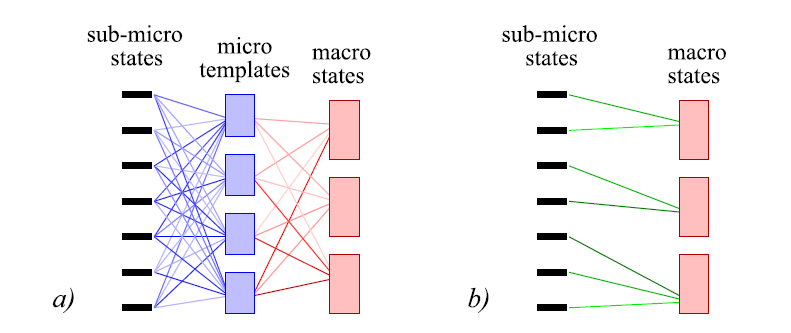
\includegraphics{images/img_4_1.png}
		}
		\caption{
		\label{i4.1}
		Классические и квантовые состояния. \textbf{a} Субмикроскопические состояния являются «скрытыми переменными». Атомы, молекулы и поля являются шаблонами, определяемыми как квантовые суперпозиции субмикроскопических состояний и используемые в общепринятом микроскопическом масштабе. Обычные <<классические>> объекты, такие как планеты и люди, являются макроскопическими, и опять же суперпозициями микро-шаблонов. Линии здесь указывают квантовые матричные элементы.  \textbf{b} Классические макроскопические состояния - вероятностные распределения субмикроскопических состояний. Здесь линии указывают вероятности. Число состояний принимает астрономические масштабы, но микроскопические шаблоны более многочисленны, чем классические, а субмикроскопических состояний и того больше.}
	\end {center}
\end {figure}

Для подхода, отстаиваемого в этой книге, было введено понятие шаблонов, представленное в разд. \ref{ch2.1}. Мы утверждаем, что обычная квантовая механика достигается, если мы выполним довольно сложное базисное преобразование в онтологических базовых состояниях. Эти новые базисные элементы, полученные таким образом, будут весьма сложными квантовыми суперпозициями онтологических состояний. Именно эти состояния мы называем <<шаблонными состояниями>>; это распознаваемые состояния, которые мы обычно используем в квантовой механике. Не исключено, что преобразование может в некоторой степени включать нелокальность.

Обращая это преобразование, можно обнаружить, что онтологические состояния, в свою очередь, будут сложными суперпозициями шаблонных состояний. Суперпозиции сложны, потому что они будут включать много мод, которые нам едва видны. Например, вакуумное состояние, наше самое элементарное шаблонное состояние, будет суперпозицией очень многих онтических (сокращенно онтологических) состояний. Почему это так, сразу становится очевидным, если мы понимаем, что вакуум является самым низким собственным состоянием гамильтониана, в то время как гамильтониан не является beable, а <<изменчивым>> (changeable) (см. Раздел \ref{ch2.1.1}). Конечно, если это верно для вакуума (раздел \ref{ch5.7.5}), он, безусловно, также будет действовать для всех других обычно используемых состояний шаблона. Мы знаем, что некоторые онтические состояния преобразуются в запутанные комбинации шаблонов, поскольку запутанные состояния могут создаваться в лаборатории.

Макроскопические состояния, которые представляют собой классические состояния, описывающие людей и планеты, а также указатели измерительного устройства и, конечно, живых и мертвых кошек, опять же являются суперпозициями шаблонных состояний в целом, но обычно они не определены с бесконечной точностью, поскольку мы не наблюдаем каждый атом внутри этих объектов. Каждое макроскопическое состояние на самом деле представляет собой композицию очень многих квантовых состояний, но они хорошо отличаются друг от друга.

На рис. \ref{i4.1} фундаментальные онтологические состояния являются субмикроскопическими, тогда мы видим микроскопические состояния, которые являются квантовыми состояниями, которые мы обычно рассматриваем, то есть матричные состояния и, наконец, макроскопические или классические состояния. Элементы матрицы, относящиеся к этим различным состояниям, обозначены линиями переменной толщины.

В предыдущем разделе утверждалось, что классические или макроскопические состояния являются диагональными в терминах субмикроскопических состояний, поэтому все они являются онтическими состояниями. Любопытно, что в Природе состояния, наиболее подходящие для описания атомов, молекул и субатомных частиц, являются шаблонными состояниями, требующими суперпозиции. Таким образом, когда мы наблюдаем классический объект, мы также смотрим на онтологические вещи, поэтому шаблонное состояние, которое мы используем для описания того, что мы ожидаем увидеть, <<коллапсирует>> в дельта-подобное распределение вероятностей в терминах классических состояний.

В беседах с коллегами автор заметил, насколько они удивлены приведенными выше утверждениями о том, что классические состояния являются онтологическими. Приведенные выше рассуждения, однако, почти невозможно игнорировать, и, действительно, наше простое наблюдение многое объясняет о том, что мы иногда воспринимаем как подлинные <<квантовые тайны>>. Таким образом, это стало неотъемлемой частью нашей теории.

\subsubsection{Вероятности}\label{ch4.3.2}

На первый взгляд может показаться, что понятие вероятности теряется в нашем подходе к квантовой механике. Наша теория является онтической, она описывает определенность, а не вероятности.

Однако вероятности возникают естественным образом и во многих классических системах. Подумайте, как ученый 19-го века смотрел бы на вероятности. В эксперименте по столкновению частиц два пучка частиц пересекаются в области взаимодействия. Как частицы будут рассеиваться? Конечно, частицы будут слишком малы, чтобы нацеливать их так точно, что мы заранее точно знали бы, как они встречаются друг с другом, поэтому мы применяем законы статистики. Без использования квантовой механики ученый 19-го века наверняка знал бы, как вычислить угловое распределение рассеянных частиц, предполагая некоторый классический потенциал взаимодействия. Происхождение статистической природы результатов его расчетов просто прослеживается в неопределенности относительно исходного состояния.

В традиционной квантовой механике начальное состояние может казаться точно известным: у нас есть два пучка, состоящих из совершенно плоских волновых функций; статистическое распределение происходит потому, что волновые функции конечного состояния имеют определенную форму, и только там квантовый физик начинает вычислять амплитуды и выводить вероятности рассеяния из них. Так что это выглядит совсем по-другому. Теперь мы собираемся объяснить, что происхождение статистики в обоих случаях в конце концов одинаково.

В нашей теории переход от классической записи к квантовой записи происходит, когда мы решаем использовать шаблонное состояние $|\psi(t)\rangle$ для описания состояния системы. При $t = 0$ коэффициенты $|\lambda_A|^2$, где (см. Замечания после уравнения (\ref{2.2}))

\begin{equation}\label{4.3}
	\left\langle\operatorname{ont}(0)_{A} | \psi(0)\right\rangle=\lambda_{A}
\end{equation}

определяют вероятность того, что мы начинаем с онтологического состояния $A$. Затем мы используем наше уравнение Шредингера для определения динамики $|\psi(t)\rangle$. Когда в какое-то время $t_1$ достигается асимптотическое превышение, мы вычисляем $\langle \mathrm{ont}(t_1)_A \mid \psi(t_1) \rangle$, где теперь онтологическое состояние представляет результат конкретного измерения, скажем, частиц, попавших в детектор под некоторым заданным углом. Согласно квантовой механике с использованием правило Борна, абсолютный квадрат этой амплитуды является вероятностью конкретного исхода, но, согласно нашей теории, начальные онтологические состояния $|\mathrm{ont}(0)_A\rangle$ развились в конечные онтологические состояния $|\mathrm{ont}(t_1)_A\rangle$, поэтому мы должны использовать те же коэффициенты $\lambda_A$. И теперь они определяют вероятность данного исхода. Таким образом, мы заключаем, что эти вероятности совпадают с вероятностями, с которых мы начали с данными онтологическими состояниями.

Конечные онтологические состояния - это онтологические состояния, которые приводят к данному результату эксперимента. Обратите внимание, что мы использовали суперпозиции при расчете амплитуд переходов, но окончательные ответы просто соответствуют вероятности того, что мы начали с данного онтологического состояния, которое, с уверенностью, превратилось в данное конечное, классическое состояние.

Наши шаблонные состояния образуют очень маленькое подмножество всех онтологических состояний, так что каждый раз, когда мы повторяем эксперимент, фактическое онтическое состояние является другим. Начальное состояние шаблона теперь представляет вероятности начальных онтических состояний, и, поскольку они проецируются в классические конечные состояния, и если начальные состояния подчиняются правилу Борна, классические конечные состояния тоже ему следуют. Следовательно, мы можем доказать, что наша теория подчиняется правилу Борна, если мы знаем, что начальное состояние делает это в отношении онтических мод. Если теперь мы постулируем, что используемые шаблонные состояния всегда отражают относительные вероятности онтических состояний теории, то правило Борна представляется неизбежным следствием [113].

Самое главное, что нет абсолютно никаких оснований пытаться включить в нашу теорию отклонения от вероятностной интерпретации Копенгагена от Борна. Правило Борна будет строго соблюдаться; то есть не будет систематических, воспроизводимых отклонений. Таким образом, мы утверждаем, что правило Борна следует из нашего требования, чтобы базис используемых нами шаблонных состояний был связан с базисом онтологических состояний посредством ортонормированного или унитарного преобразования.

Таким образом, мы получили, что: пока мы используем ортонормированные преобразования для перехода от одного базиса к другому, правило Борна, включая использование абсолютных квадратов для представления вероятностей, является единственным правильным выражением для этих вероятностей.



\end{document}